\section{Interfejs użytkownika (Zofia Sosińska)}\label{chap:ui}
Interfejs użytkownika (ang. user interface, UI)jest to zbiór najważniejszych informacji przedstawiony graczowi w sposób czytelny. Może się to odbywać za pomocą na przykład obrazków, tekstów, czy wskaźników. Dzięki UI możliwy jest wgląd w aktualny stan wiedzy grywalnej postaci. 
Projekt interfejsu użytkownika przewiduje trzy tryby: zwykły, budowania oraz walki. Zadaniem każdego z nich będzie odzwierciedlenie aktualnej wiedzy granej postaci z naciskiem na najpotrzebniejsze w danej chwili informacje.
	
\subsubsection{Tryb zwykły}
Tryb zwykły przewiduje podstawowe funkcje, takie jak pokazanie:
surowców i funduszy,
aktualnego czasu w grze, 
kompasu,
ikony postaci, na które gracz może się przełączyć;
Inspiracją dla górnego paska z informacjami oraz dla ikon dostępnych postaci jest ten użyty w grze Warcraft 3. Prostota i surowość użytego stylu będą współgrać z klimatem gry.

\begin{figure}[htbp]
    \centering
    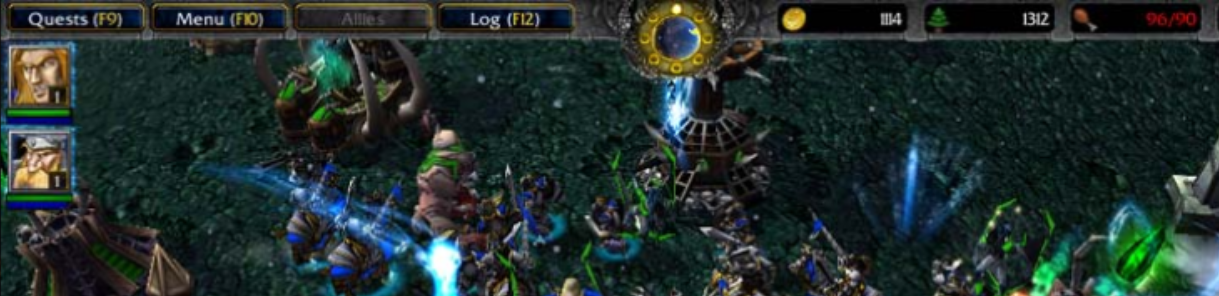
\includegraphics[width=0.9\textwidth]{images/ui/warcraft3.png}
    \caption{Pasek z informacjami oraz dla ikony dostępnych postaci w grze Warcraft 3.}\label{fig:Warcraft3}
\end{figure}

W naszej grze skupimy się jednak na tym, aby interfejs użytkownika zabierał jak najmniej miejsca. Dlatego też projekt zakłada, że poszczególne obiekty nie będą ze sobą połączone, a jedynie “dryfować” w przestrzeni.
Jako ważny element tej części UI zawarty zostanie kompas, wzorowany na tym z gry The Elder Scrolls V: Skyrim.

\begin{figure}[htbp]
    \centering
    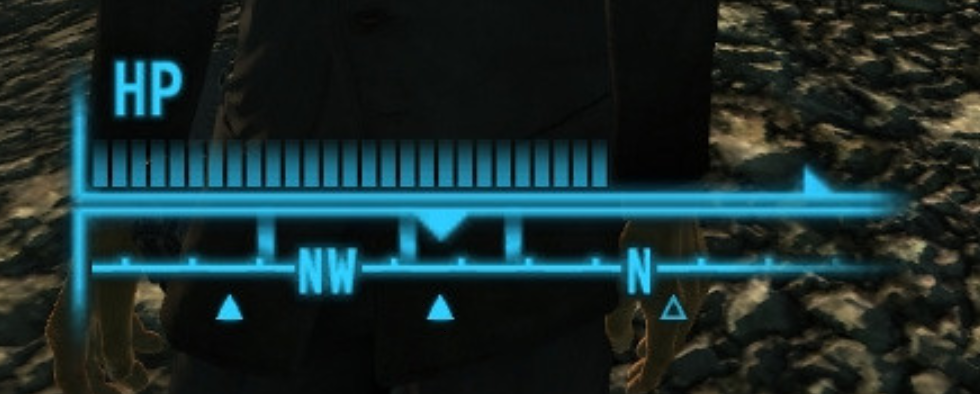
\includegraphics[width=0.9\textwidth]{images/ui/compassSkyrim.png}
    \caption{Kompas z gry Skyrim}\label{fig:Fallout}
\end{figure}

Szacowany projekt trybu zwykłego UI wyświetlono na rysunku \ref{fig:ui_main} .
\begin{figure}[htbp]
    \centering
    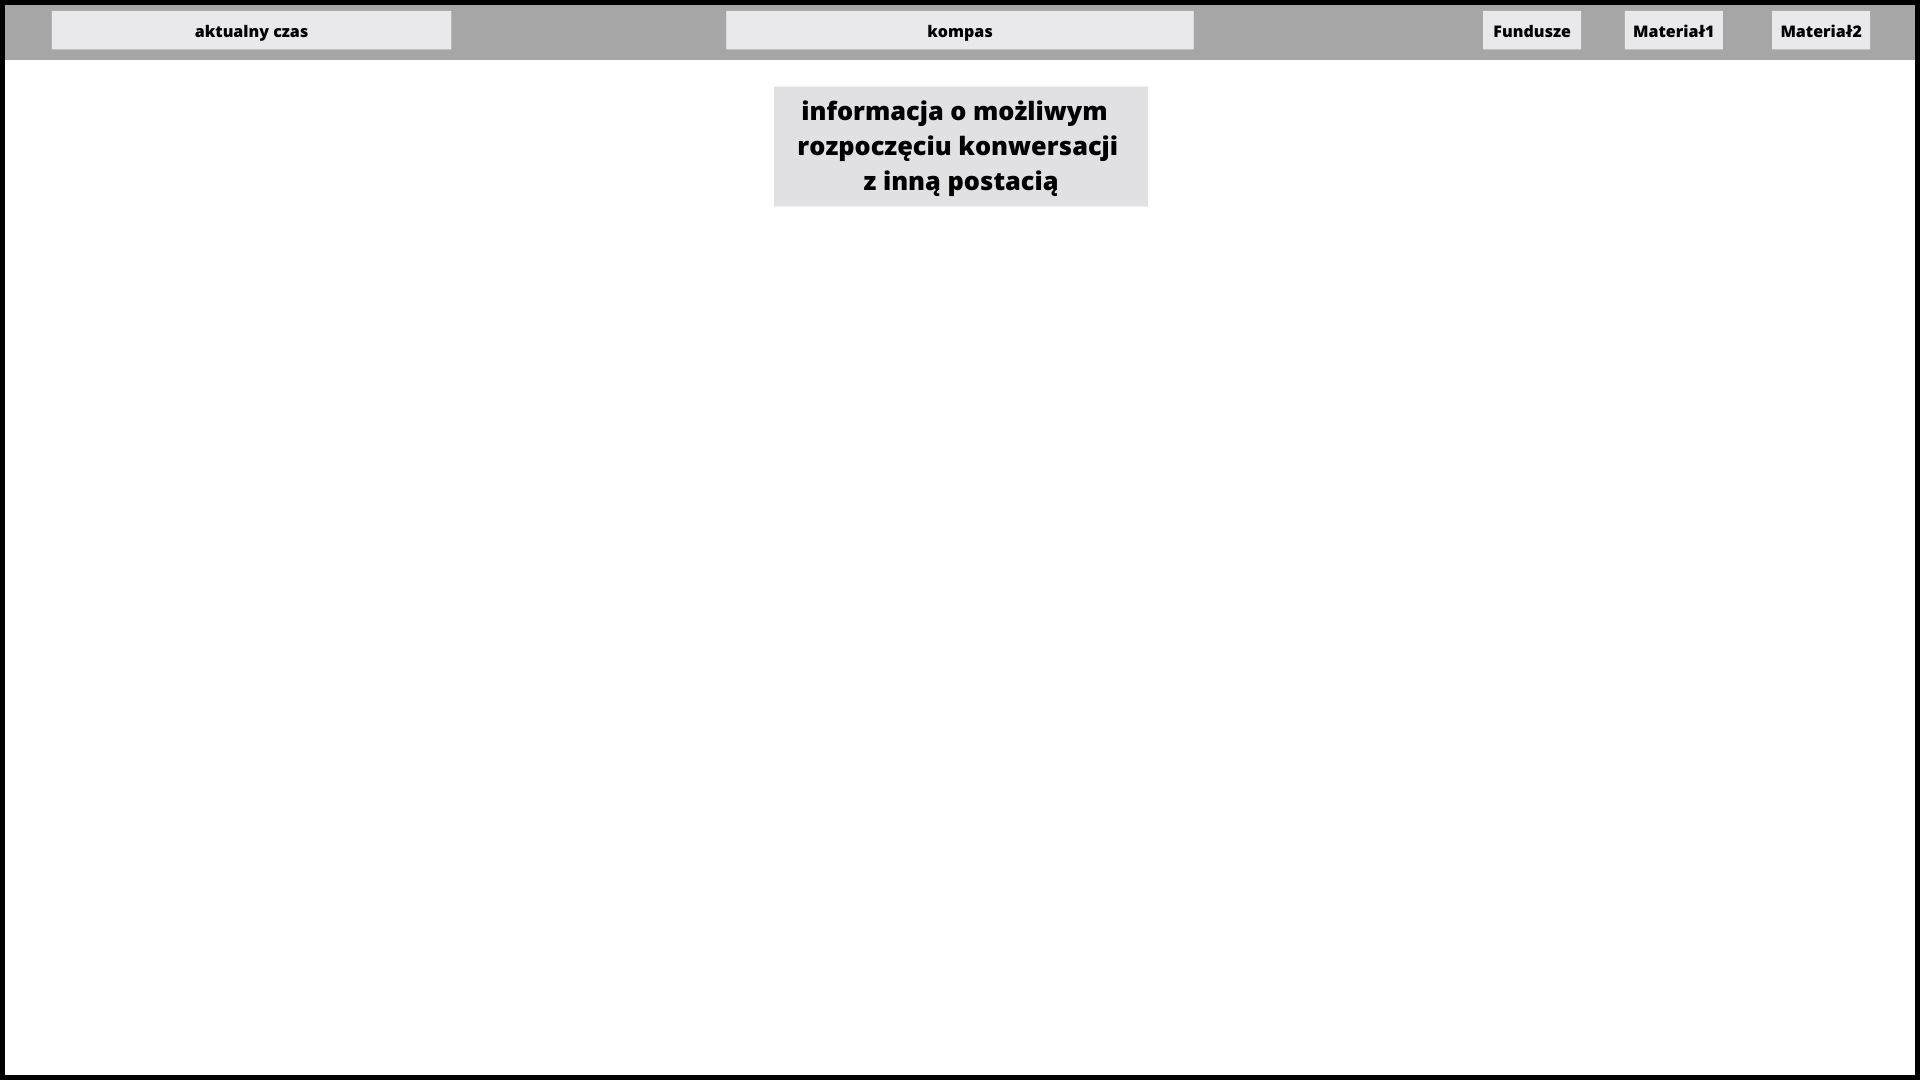
\includegraphics[width=0.9\textwidth]{images/ui/ui_proj_ogolne.jpg}
    \caption{Projekt trybu zwykłego UI.
    }\label{fig:ui_main}
\end{figure}
 
\subsubsection{Tryb budowania}
 W trybie budowania informacje wcześniej przedstawione zostaną na ekranie. Dodatkowo pokażą nam się dostępne do zbudowania budynki, a po wybraniu pojawią się przed nami. Po zatwierdzeniu budynek zostanie wybudowany.
	Inspiracją do przedstawienia dostępnych budowli jest rozwiązanie gry Orcs must die!

    \begin{figure}[h!tbp]
        \centering
        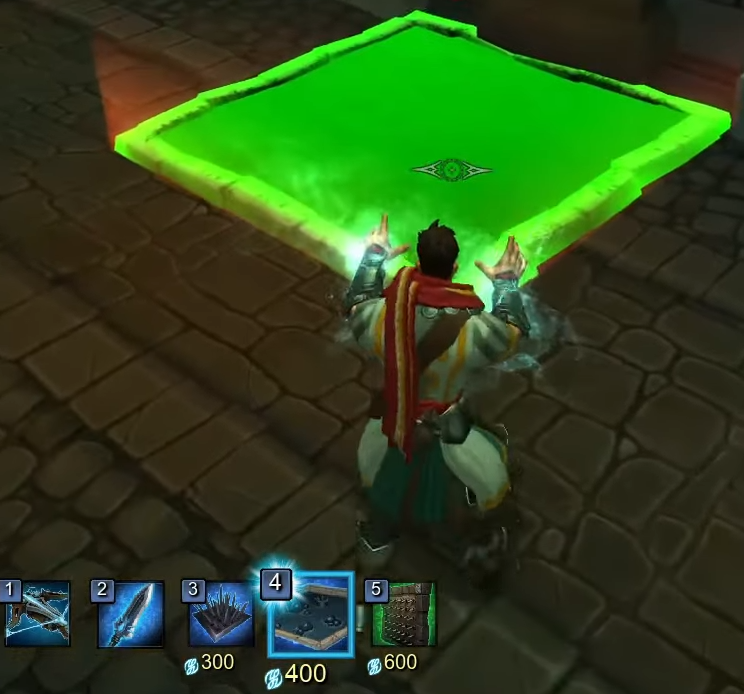
\includegraphics[width=0.5\textwidth]{images/ui/buoildingsOrcs.png}
        \caption{Wyświetlenie dostępnych pułapek w Orcs must die!}\label{fig:Orcs}
    \end{figure}

    Szacowany projekt trybu budowania UI wyświetlono na rysunku \ref{fig:ui_bud} .
    \begin{figure}[htbp]
        \centering
        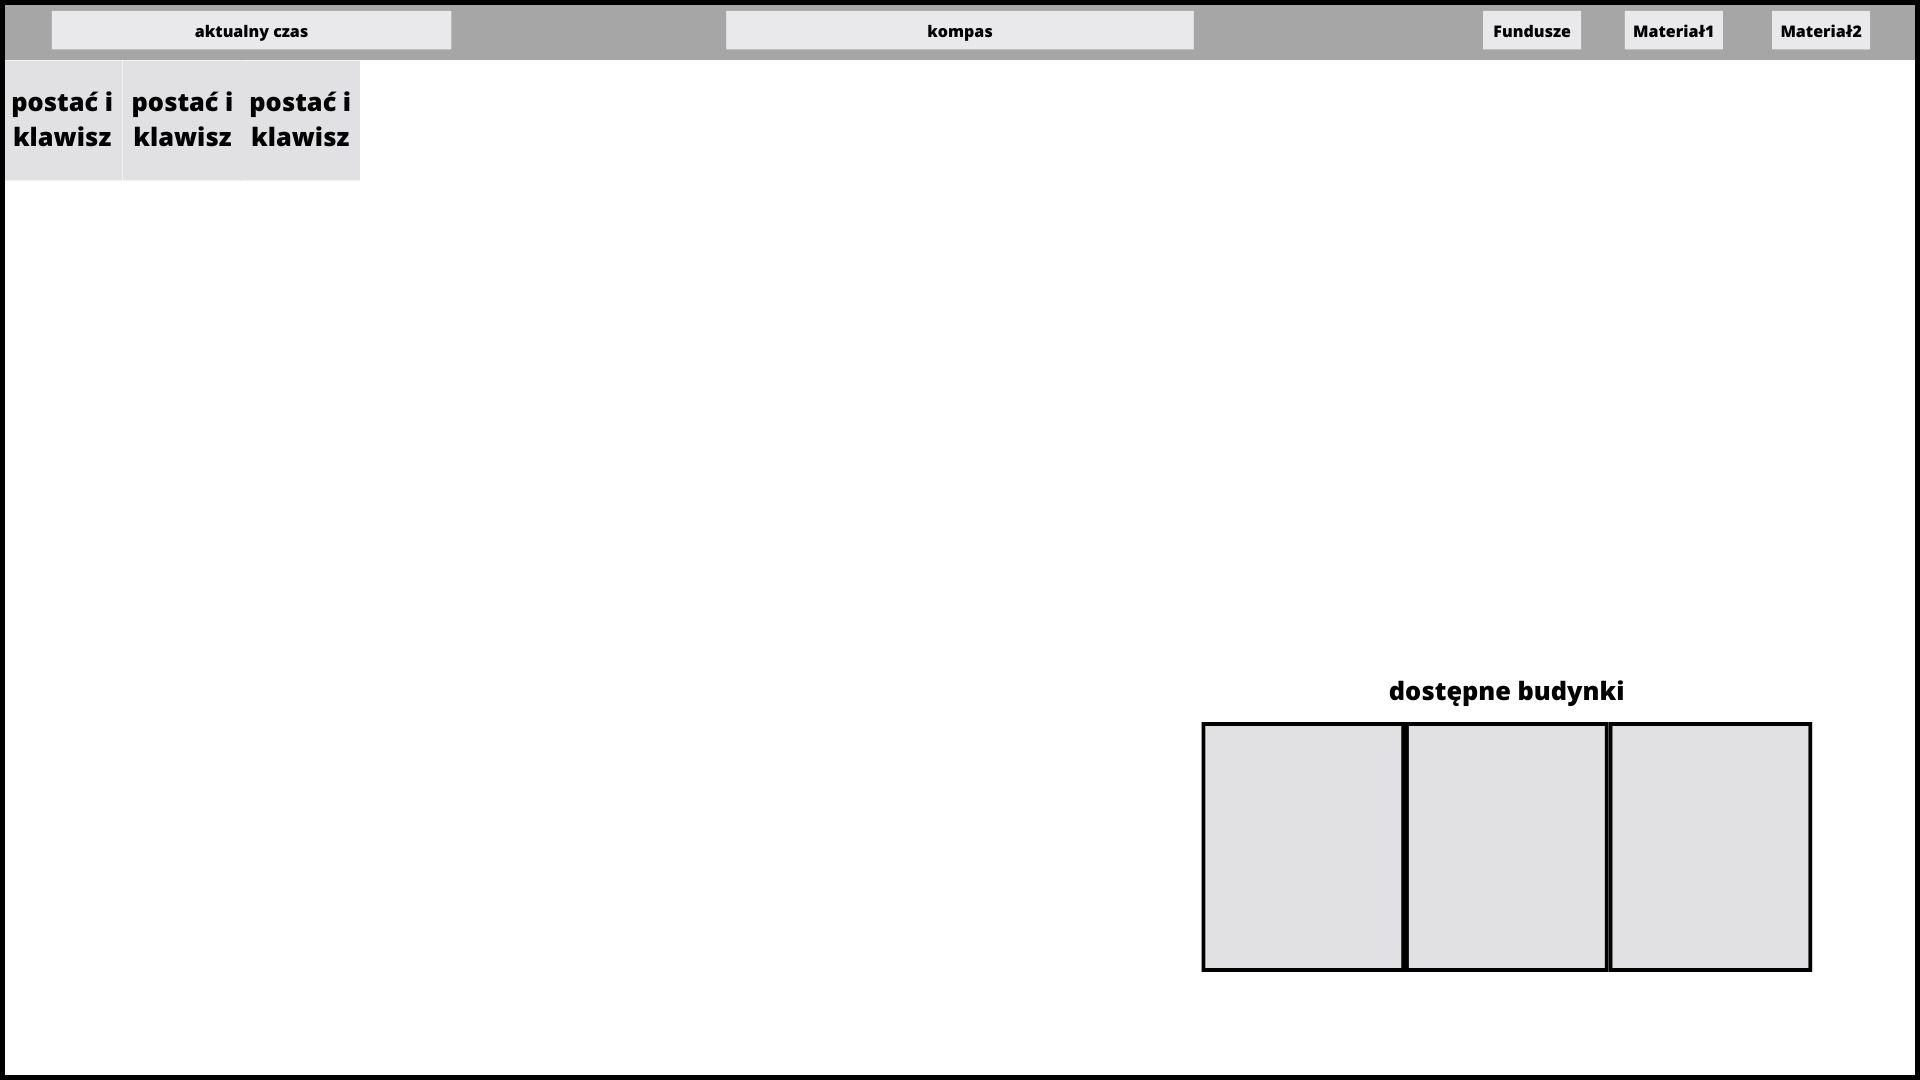
\includegraphics[width=0.9\textwidth]{images/ui/ui_proj_budowanie.jpg}
        \caption{Projekt trybu budowania UI.
        }\label{fig:ui_bud}
    \end{figure}


\subsubsection{Tryb walki}
Bliźniaczo do trybu budowania, gdy rozpocznie się walka, podstawowe informacje zostają na ekranie, a dodatkowo gracz dostaje informacje o dostępnych rozkazach do wydania. Nasze rozwiązanie będzie podobne do pomysłu z gry Mount\&Blade.

\begin{figure}[h!tbp]
    \centering
    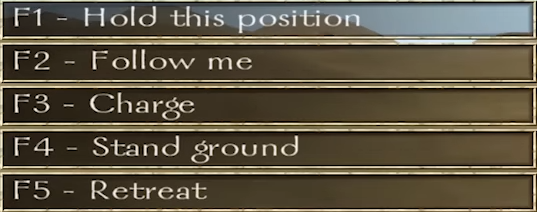
\includegraphics[width=0.9\textwidth]{images/ui/commandsMountBla.png}
    \caption{Wykaz dostępnych rozkazów z gry Mount\&Blade.}\label{fig:MountnBlade}
    \label{fig:mnb}
\end{figure}

Szacowany projekt trybu budowania UI wyświetlono na rysunku \ref{fig:ui_wal} .
    \begin{figure}[htbp]
        \centering
        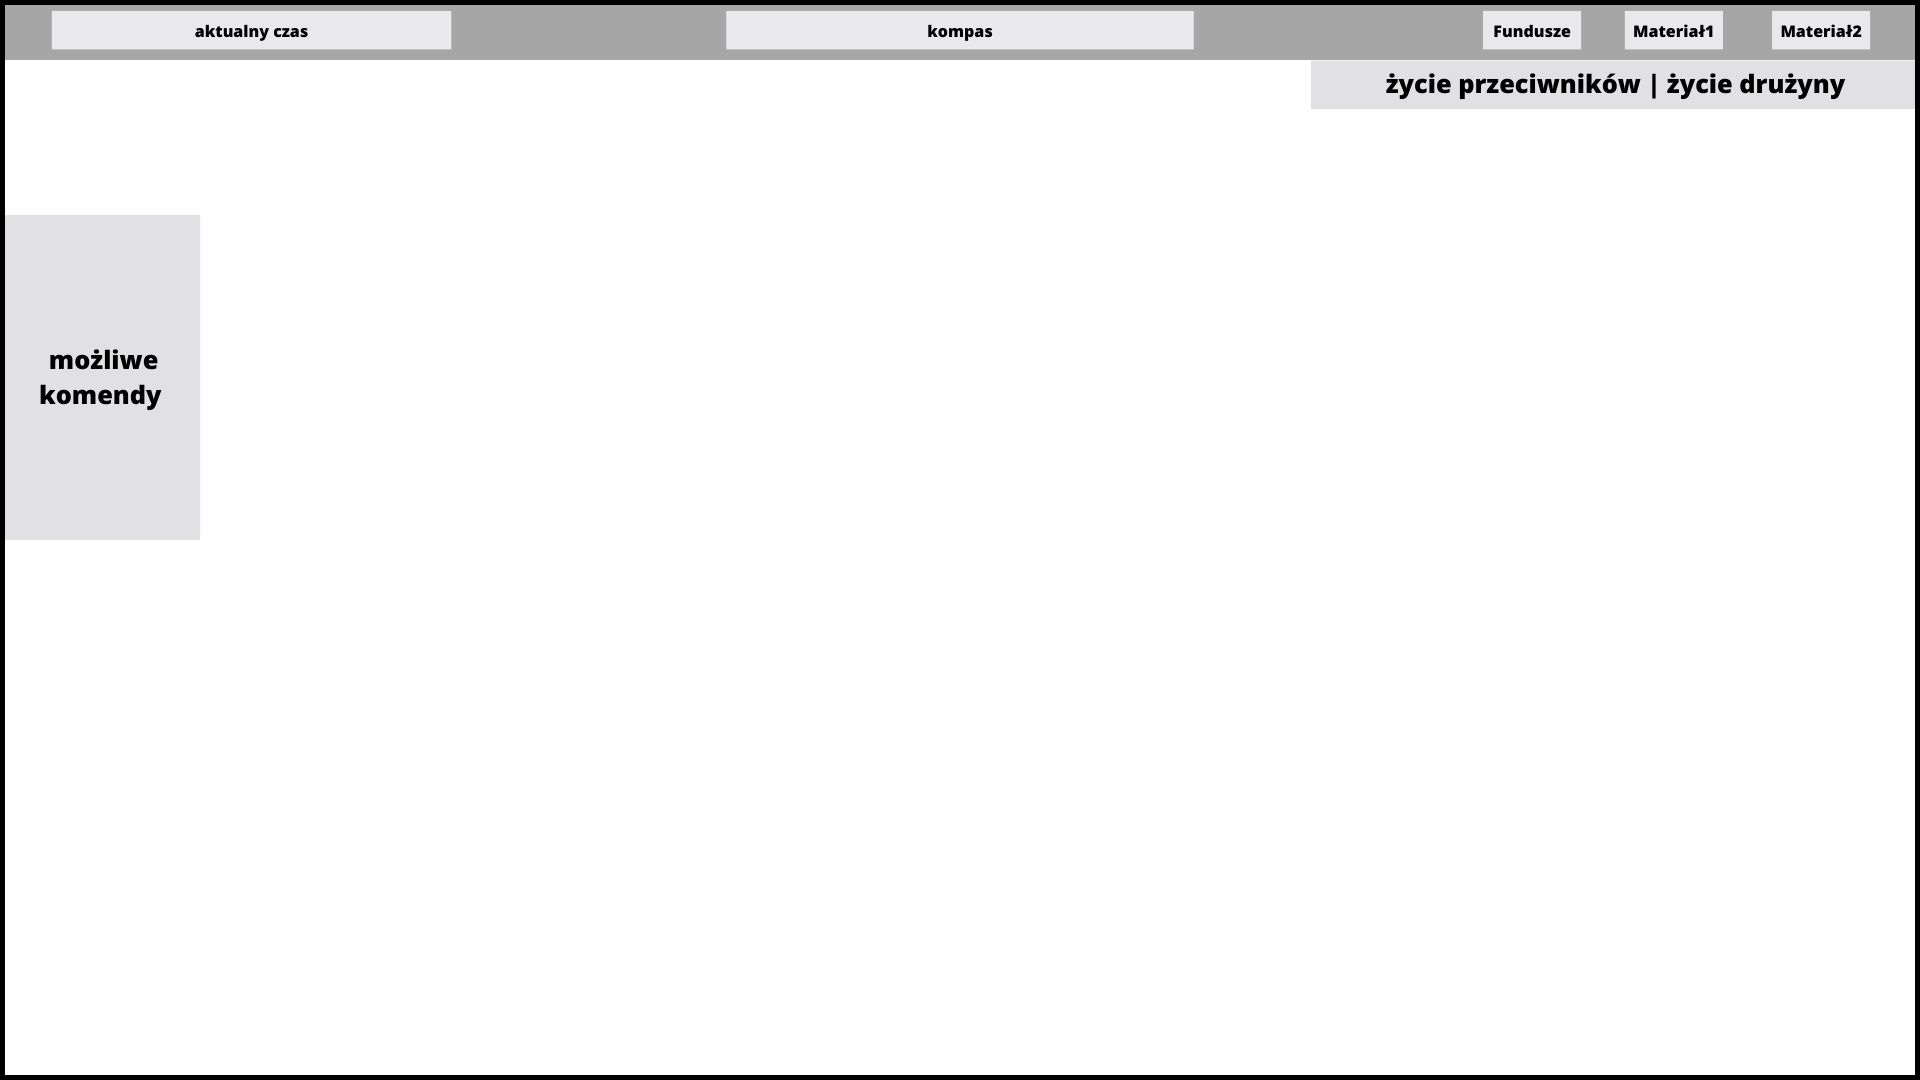
\includegraphics[width=0.9\textwidth]{images/ui/ui_proj_walka.jpg}
        \caption{Projekt trybu walki UI.
        }\label{fig:ui_wal}
    \end{figure}
